\documentclass[10pt]{article}
\usepackage[margin=0.7in]{geometry}
\usepackage{amsmath,amssymb,mathtools}
\usepackage{tikz}
\usetikzlibrary{arrows.meta,calc}
\usepackage{hyperref}

\newcommand{\cA}{\cos\alpha}
\newcommand{\sA}{\sin\alpha}
\newcommand{\cB}{\cos\beta}
\newcommand{\sB}{\sin\beta}
\newcommand{\cG}{\cos\gamma}
\newcommand{\sG}{\sin\gamma}
\newcommand{\vect}[1]{\boldsymbol{#1}}

\title{Why Euler Angles Have Gimbal Lock\\\large Yuqing Yang}
\author{}
\date{}

\begin{document}
\maketitle
\vspace{-1.4em}

When describing rotation in the space, we usually rotate for three times. First, rotate with axis x, then y, then axis z.

If we can describe each rotation as a matrix $R_x, R_y, R_z$, a vector $\vect x$ will be transformed to $R_z R_y R_x \vect x$.
% \paragraph{Convention.}
% Vectors are column vectors and every matrix below is an \emph{active}
% rotation: it moves the vector while the coordinate axes stay fixed.  We use
% the order ``first $x$, then $y$, then $z$.''  Therefore the matrix nearest the
% vector acts first.  Angles are written in radians in the formulas; $90^{\circ}$
% means $\pi/2$.

\section*{1. A clockwise rotation in the $xy$-plane}

\begin{center}
  % Requires: \usepackage{tikz}
%           \usetikzlibrary{arrows.meta}

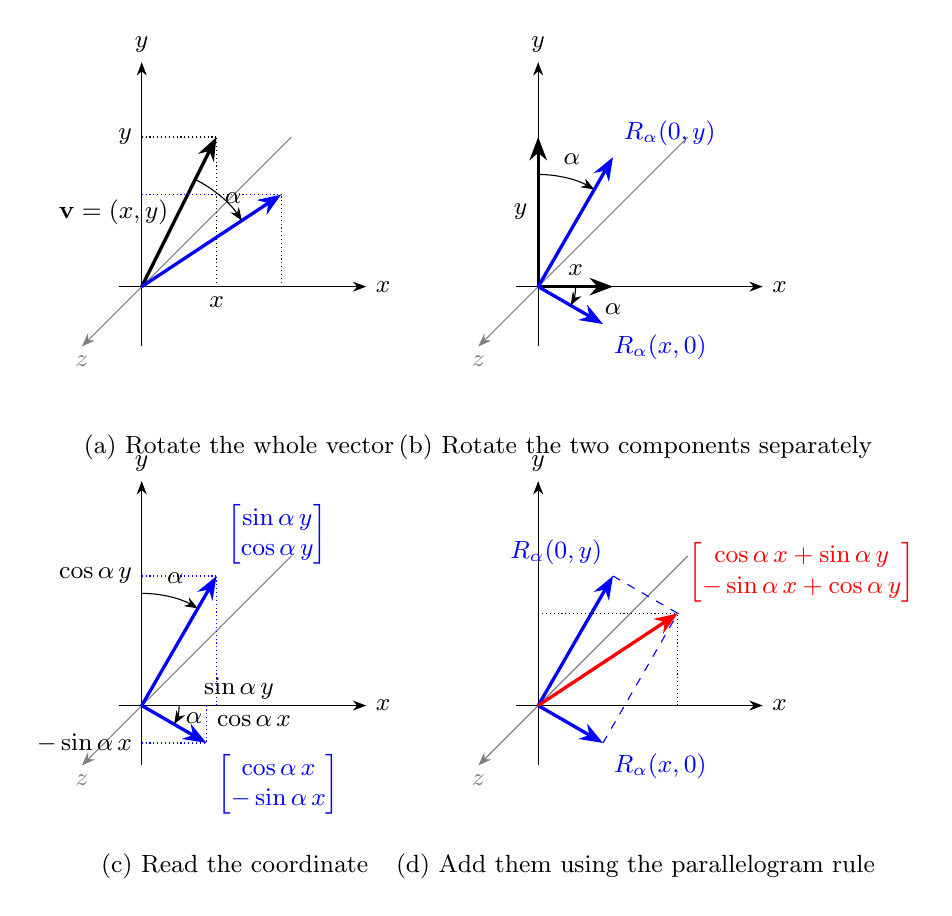
\begin{tikzpicture}[
  >=Stealth,
  scale=0.95,
  every node/.style={font=\small},
  original/.style={very thick,->},
  rotated/.style={very thick,blue,->},
  guide/.style={densely dotted},
  blueguide/.style={densely dotted,blue}
]

% Numerical illustration: x=1, y=2, alpha=30 degrees.
% Rotated endpoint: (1.866, 1.232).

% ------------------------------------------------------------
% (a) Original vector and its rotated image
% ------------------------------------------------------------
\begin{scope}
  \draw[->] (-0.3,0)--(3.0,0) node[right] {$x$};
  \draw[->] (0,-0.8)--(0,3.0) node[above] {$y$};
  \draw[gray,->] (2,2)--(-0.8,-0.8) node[below] {$z$};


  \draw[original] (0,0)--(1,2) node[midway,left] {$\mathbf v=(x,y)$};
  \draw[guide] (1,0)--(1,2);
  \draw[guide] (0,2)--(1,2);
  \node[below] at (1,0) {$x$};
  \node[left] at (0,2) {$y$};

  \draw[rotated] (0,0)--(1.866,1.232);
  \draw[blueguide] (1.866,0)--(1.866,1.232);
  \draw[blueguide] (0,1.232)--(1.866,1.232);

  \draw[->] (0.72,1.43) arc[start angle=63.4,end angle=33.4,radius=1.6];
  \node at (1.22,1.18) {$\alpha$};

  \node[align=center] at (1.3,-2.15) {(a) Rotate the whole vector};
\end{scope}

% ------------------------------------------------------------
% (b) Split into x- and y-components, then rotate each
% ------------------------------------------------------------
\begin{scope}[xshift=5.3cm]
  \draw[->] (-0.3,0)--(3.0,0) node[right] {$x$};
  \draw[->] (0,-0.8)--(0,3.0) node[above] {$y$};
  \draw[gray,->] (2,2)--(-0.8,-0.8) node[below] {$z$};


  % Original components
  \draw[original] (0,0)--(1,0) node[midway,above] {$x$};
  \draw[original] (0,0)--(0,2) node[midway,left] {$y$};

  % Rotated x-component
  \draw[rotated] (0,0)--(0.866,-0.5)
    node[below right] {$R_\alpha(x,0)$};
  \draw[->] (0,1.5) arc[start angle=90,end angle=60,radius=1.5];
  \node at (0.45,1.7) {$\alpha$};
  % Rotated y-component
  \draw[rotated] (0,0)--(1,1.732)
    node[above right] {$R_\alpha(0,y)$};
  \draw[->] (0.5,0) arc[start angle=0,end angle=-30,radius=0.5];
  \node at (1,-0.3) {$\alpha$};
  \node[align=center] at (1.3,-2.15)
    {(b) Rotate the two components separately};
\end{scope}

% ------------------------------------------------------------
% (c) Coordinate contributions of the rotated components
% ------------------------------------------------------------
\begin{scope}[yshift=-5.6cm]
  \draw[->] (-0.3,0)--(3.0,0) node[right] {$x$};
  \draw[->] (0,-0.8)--(0,3.0) node[above] {$y$};
  \draw[gray,->] (2,2)--(-0.8,-0.8) node[below] {$z$};


  % Rotated x-component
  \draw[rotated] (0,0)--(0.866,-0.5) node [below right, align=left]{$\displaystyle
      \begin{bmatrix}
        \cos\alpha\,x\\
        -\sin\alpha\,x
      \end{bmatrix}$};

  \draw[blueguide] (0.866,0)--(0.866,-0.5);
  \draw[blueguide] (0,-0.5)--(0.866,-0.5);
  \node[below] at (1.5,0) {$\cos\alpha\,x$};
  \node[left] at (0,-0.5) {$-\sin\alpha\,x$};

  % Rotated y-component
  \draw[rotated] (0,0)--(1,1.732) node [above right, align=left]{$\displaystyle
      \begin{bmatrix}
        \sin\alpha\,y\\
        \cos\alpha\,y
      \end{bmatrix}$};

  \draw[blueguide] (1,0)--(1,1.732);
  \draw[blueguide] (0,1.732)--(1,1.732);
  \node[below] at (1.3,0.5) {$\sin\alpha\,y$};
  \node[left] at (0,1.732) {$\cos\alpha\,y$};
  \draw[->] (0,1.5) arc[start angle=90,end angle=60,radius=1.5];
  \node at (0.45,1.7) {$\alpha$};
  \draw[->] (0.5,0) arc[start angle=0,end angle=-30,radius=0.5];
  \node at (0.7,-0.175) {$\alpha$};
  \node[align=center] at (1.3,-2.15)
    {(c) Read the coordinate };
\end{scope}

% ------------------------------------------------------------
% (d) Add the rotated components with a parallelogram
% ------------------------------------------------------------
\begin{scope}[xshift=5.3cm,yshift=-5.6cm]
  \draw[->] (-0.3,0)--(3.0,0) node[right] {$x$};
  \draw[->] (0,-0.8)--(0,3.0) node[above] {$y$};
  \draw[gray,->] (2,2)--(-0.8,-0.8) node[below] {$z$};

  % Two rotated components
  \draw[rotated] (0,0)--(0.866,-0.5)
    node[below right] {$R_\alpha(x,0)$};
  \draw[rotated] (0,0)--(1,1.732)
    node[above left] {$R_\alpha(0,y)$};

  % Parallelogram sides
  \draw[blue,dashed] (0.866,-0.5)--(1.866,1.232);
  \draw[blue,dashed] (1,1.732)--(1.866,1.232);

  % Final sum
  \draw[very thick,red,->] (0,0)--(1.866,1.232)
    node[above right,align=left] {$\displaystyle
      \begin{bmatrix}
        \cos\alpha\,x+\sin\alpha\,y\\
        -\sin\alpha\,x+\cos\alpha\,y
      \end{bmatrix}$};

  \draw[guide] (1.866,0)--(1.866,1.232);
  \draw[guide] (0,1.232)--(1.866,1.232);

  \node[align=center] at (1.3,-2.15)
    {(d) Add them using the parallelogram rule};
\end{scope}

\end{tikzpicture}
\end{center}

Suppose we have a paper in front of us, and we look into the paper. There is a vertical z axis that points at our nose, because we usually define z axis as straight-up. When we look down, we are looking at an axis pointing at our nose. For now, let's forget about z axis and focus on xy plane.


As shown in a), let $\vect v=(x,y)^T$. This can be decomposed as:
\[
  \vect v=\begin{bmatrix}x\\0\end{bmatrix}
          +\begin{bmatrix}0\\y\end{bmatrix}.
\]

As shown in b, rotating the original $\vect v$ is equivalent to rotating the two component vectors for $\alpha$ degrees.


As shown in c), after a clockwise rotation by $\alpha$, the first part contributes
$(x\cos\alpha,-x\sin\alpha)^T$, while the second contributes
$(y\sin\alpha,y\cos\alpha)^T$.  

As shown in d), adding them gives
\[
 \begin{bmatrix}x'\\y'\end{bmatrix}
 =\begin{bmatrix}
     \cos\alpha\,x+  \sin\alpha\,y\\
    -\sin\alpha\,x+ \cos\alpha\,y
   \end{bmatrix}
 =\begin{bmatrix}
     \cos\alpha & \sin\alpha\\
    -\sin\alpha & \cos\alpha
   \end{bmatrix}
   \begin{bmatrix}x\\y\end{bmatrix}.
\]

Thus this matrix is the transformation for rotating $\alpha$ degrees clockwise:

\[
\begin{bmatrix}
     \cos\alpha & \sin\alpha\\
    -\sin\alpha & \cos\alpha
   \end{bmatrix}
\]

However, because we are now looking at the direction where z points at out nose. This means that we observe against the direction of z axis. To unify in mathematics, we want to look following the direction of z axis. So I have to be behind our screen and look towards you. 

We will discuss in appendix that, when we swap sides (following $+z$ direction instead of $-z$ direction), clockwise rotation becomes counter clockwise. So the angle $\alpha$ becomes a negation $-\alpha$.

Thus, the matrix should be 

\[
\begin{bmatrix}
     \cos(-\alpha) & \sin(-\alpha)\\
    -\sin(-\alpha) & \cos(-\alpha)
   \end{bmatrix}
\sim
   \begin{bmatrix}
     \cos\alpha & -\sin\alpha\\
    \sin\alpha & \cos\alpha
   \end{bmatrix}
\]


\section*{2. The same idea in three dimensions}
Because rotating $(x,y,z)^T$ about the $z$-axis changes only its $x$ and $y$
coordinates.  Hence
\[
 R_z(\gamma)\begin{bmatrix}x\\y\\z\end{bmatrix}
 =\begin{bmatrix}\cG{}x-\sG{}y\\\sG{}x+\cG{}y\\z\end{bmatrix},\qquad
 R_z(\gamma)=
 \begin{bmatrix}
 \cG&-\sG&0\\
 \sG&\cG&0\\
 0&0&1
 \end{bmatrix}.
\]
The $1$ leaves $z$ unchanged.  The other zeros say that $z$ does not participate in the new $x$ or $y$, and that $x,y$ do not participate in the new $z$. 

\textbf{Look at the top left 2x2 partition!} This is exactly what we had in the last paragraph.

For the Euler-angle convention used in this note, take
\[
 R_x(\alpha)=
 \begin{bmatrix}1&0&0\\0&\cA&-\sA\\0&\sA&\cA\end{bmatrix},\qquad
 R_y(\beta)=
 \begin{bmatrix}\cB&0&\sB\\0&1&0\\-\sB&0&\cB\end{bmatrix},\qquad
 R_z(\gamma)=
 \begin{bmatrix}\cG&-\sG&0\\\sG&\cG&0\\0&0&1\end{bmatrix}.
\]
The signs attached to a named angle depends how we define "clockwise"; Appendix~A explains
the apparent sign change for a rotation about the $y$-axis. But we do not have to worry about this. Just apply these matrices is sufficient.

\section*{3. Compose the rotations}

To rotate a vector first about $x$ by $\alpha$, then about $y$ by $\beta$,
and finally about $z$ by $\gamma$, use
\[
 \vect v_{\rm final}=R_z(\gamma)R_y(\beta)R_x(\alpha)\vect v.
\]
The right-to-left order is essential.  Multiplying step by step,
\[
 R_y(\beta)R_x(\alpha)=
 \begin{bmatrix}
 \cB&\sA\sB&\cA\sB\\
 0&\cA&-\sA\\
 -\sB&\sA\cB&\cA\cB
 \end{bmatrix},
\]
and therefore
\[
\begin{aligned}
 R(\alpha,\beta,\gamma)
 &=R_z(\gamma)R_y(\beta)R_x(\alpha)\\[0.25em]
 &=\begin{bmatrix}
 \cG\cB & \cG\sB\sA-\sG\cA & \cG\sB\cA+\sG\sA\\
 \sG\cB & \sG\sB\sA+\cG\cA & \sG\sB\cA-\cG\sA\\
 -\sB & \cB\sA & \cB\cA
 \end{bmatrix}.
\end{aligned}
\]

\section*{4. Gimbal lock at $\beta=90^\circ$}

Set $\beta=\pi/2$, so that $\cB=0$ and $\sB=1$.  The composite matrix
becomes
\[
 R\left(\alpha,\frac\pi2,\gamma\right)=
 \begin{bmatrix}
 0&\sA\cG-\cA\sG&\cG\cA+\sG\sA\\
 0&\cA\cG+\sA\sG& -\sA\cG+\cA\sG\\
 -1&0&0
 \end{bmatrix}.
\]
Using the angle-subtraction identities gives the revealing form
\[
 \boxed{
 R\left(\alpha,\frac\pi2,\gamma\right)=
 \begin{bmatrix}
 0&\sin(\alpha-\gamma)&\cos(\alpha-\gamma)\\
 0&\cos(\alpha-\gamma)& -\sin(\alpha-\gamma)\\
 -1&0&0
 \end{bmatrix}.}
\]
Only $\gamma-\alpha$ remains.  For example, replacing
$(\alpha,\gamma)$ by $(\alpha+t,\gamma+t)$ leaves the matrix exactly
unchanged for every $t$.  Two nominally independent rotations have become
one rotation about the same effective axis: one degree of freedom has been
lost.  This is \emph{gimbal lock}.  It is a singularity of this Euler-angle
parameterization, not a loss of possible physical orientations.

\appendix
\section*{Appendix A. Why the sign for a $y$-rotation can look reversed}

``Clockwise'' is meaningful only after choosing a viewing direction. \textbf{If we define clockwise rotation as positive angle ($+30^\circ$)}: an
observer looking along $-z$ toward the origin sees the $xy$-plane (left figure) sees the angle being clockwise from y towards right bottom.

An observer looking along $+z$ sees the $xy$ plaine with x towards left instead of right (right figure). The angle is towards left bottom. The angle becomes counter-clockwise into $-30^\circ$!


\begin{center}
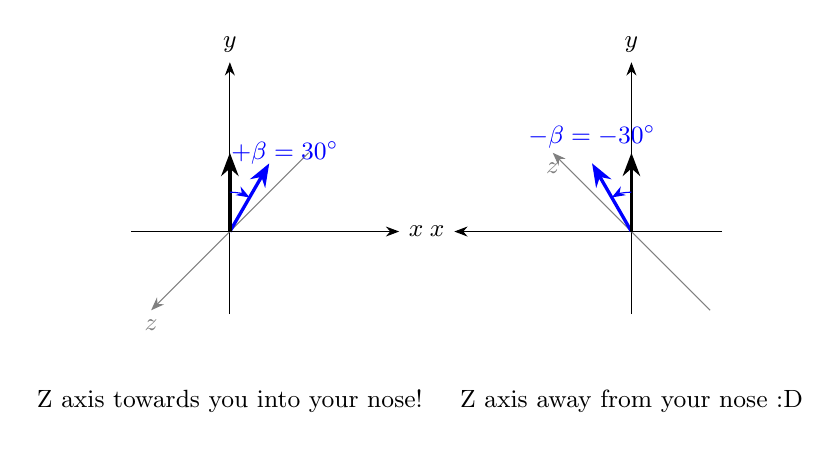
\begin{tikzpicture}[>=Stealth,scale=1.0, every node/.style={font=\small}]
  \begin{scope}
    \draw[->] (-1.25,0)--(2.15,0) node[right] {$x$};
    \draw[->] (0,-1.05)--(0,2.15) node[above] {$y$};
    \draw[gray,->] (1,1)--(-1,-1) node[below] {$z$};

    \draw[very thick,blue,->] (0,0)--(0.5,0.866);
    \draw[very thick,black,->] (0,0)--(0,1);
    \draw[blue,->] (0,0.5) arc [start angle=90, end angle=60, radius=0.5];
    \node[blue] at (0.7,1) {$+\beta =30^\circ$};
    % \node[align=center] at (0,-1.65) {View along $+y$\\toward the origin};
    % \draw[->,gray] (0,1.52)--(0,1.25) node[midway,right] {$+y$ view};
    \node[align=center] at (0,-2.15)
    {Z axis towards you into your nose!};
  \end{scope}
  \begin{scope}[xshift=5.1cm]
    \draw[->] (1.15,0)--(-2.25,0) node[left] {$x$};
    \draw[->] (0,-1.05)--(0,2.15) node[above] {$y$};
    \draw[gray,->] (1,-1)--(-1,1) node[below] {$z$};

    \draw[very thick,blue,->] (0,0)--(-0.5,0.866);
    \draw[very thick,black,->] (0,0)--(0,1);
    \draw[blue,->] (0,0.5) arc [start angle=90, end angle=120, radius=0.5];
    \node[blue] at (-0.5,1.2) {$-\beta =-30^\circ$};
    \node[align=center] at (0,-2.15)
    {Z axis away from your nose :D};
  \end{scope}
\end{tikzpicture}
\end{center}


Changing views have changed how we view clockwise, but the rotation is the same. So depending on whether we view as we see the screen, or we view as we stand behind the screen and look towards \textit{you}, the angle may be positive or negative. If we swap sides, we simply replace $\beta$ by
$-\beta$; cos is unchanged and sin changes sign.

\[
R_y(\beta)=
 \begin{bmatrix}\cB&\sB\\-\sB&\cB\end{bmatrix},\qquad
R_y(-\beta)=
\begin{bmatrix}\cB&-\sB\\\sB&\cB\end{bmatrix},\qquad
\]

Again, the rotation is the same. It is just how we define a positive angle and where we stand respectively matters. Conventionally, in mathematics, we only revert the rotation about axis y into the second form, and keep x and z. To remember this, it is a pattern like "+", "-", "+", "-", ...

This pattern is interesting because it will occur more frequently when we get into determinants.

\end{document}
